\documentclass[11pt]{exam}

\usepackage{amsmath}
\usepackage{graphicx}
\usepackage{geometry}
\usepackage{etoolbox}
\BeforeBeginEnvironment{choices}{\par\nopagebreak\minipage{\linewidth}}
\AfterEndEnvironment{choices}{\endminipage}
\geometry{
a4paper,
total={185mm,257mm},
left=10mm,
top=25mm,
bottom=10mm
}

\begin{document}
\setlength{\voffset}{-0.5in}
\setlength{\headsep}{5pt}

\fbox{\fbox{\parbox{8cm}{\centering
\vspace{2mm}
Testat - Versuch K - Radioaktivitaet - 2
\vspace{2mm}
}}}
\hspace{2mm}
\makebox[0.25\textwidth]{Name:\enspace\hrulefill} \hspace{5mm}
\makebox[0.2\textwidth]{Datum:\enspace\hrulefill}
\vspace{4mm}

\begin{questions}

\question Wie lautet die Einheit der physikalischen Größe Aktivität?

\begin{choices}
	\choice Gray (Gy)
	\choice Meter (m)
	\choice Joule (J)
	\choice Becquerel (Bq) (correct)
	\choice Zeit (t)
\end{choices}

\vspace{3mm}\question Im unten dargestellten Diagramm ist die gemessene Zählrate eines radioaktiven Präparates in Abhängigkeit von der Zeit dargestellt. Wie groß ist die Halbwertszeit?

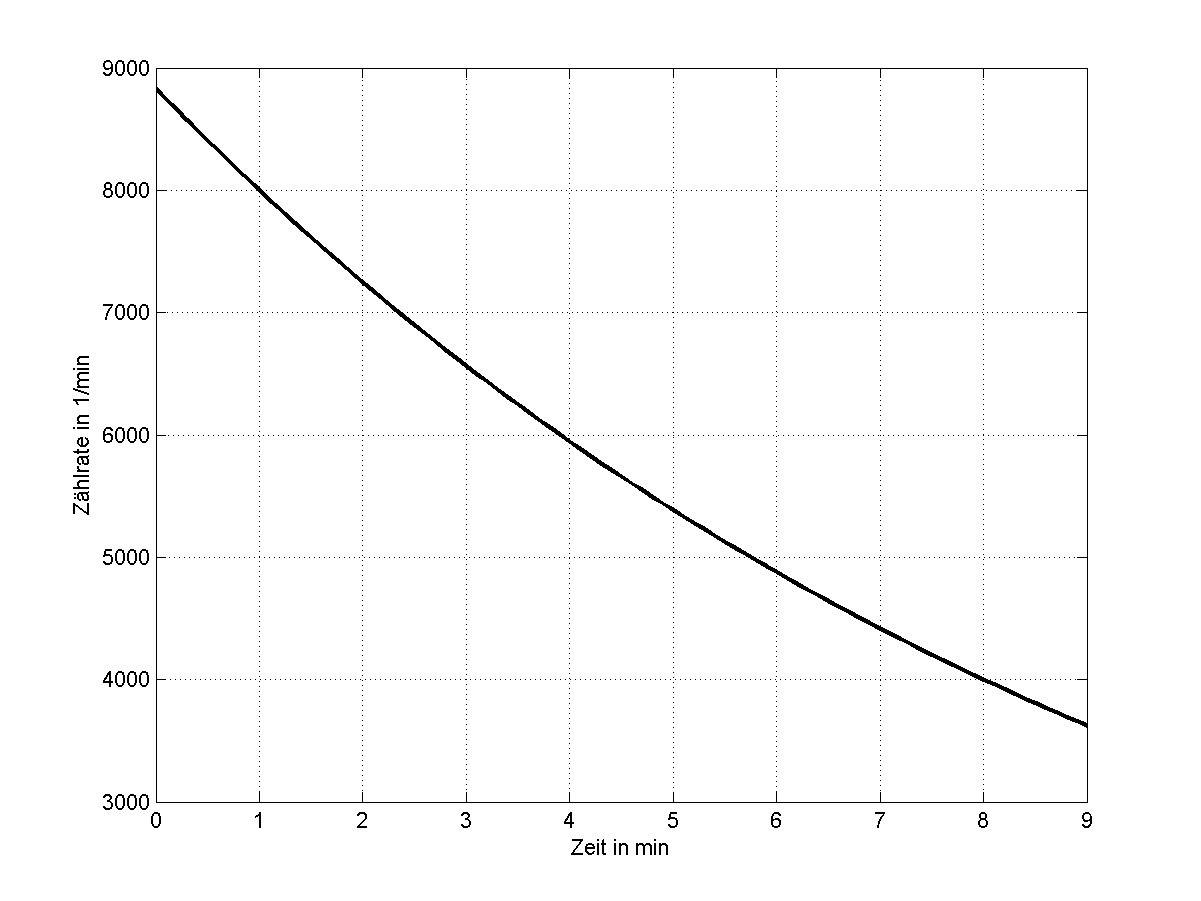
\includegraphics[width=0.5\textwidth]{../../../questions/K/images/zerfall2.png}

\begin{choices}
	\choice etwa 5 min
	\choice etwa 6 min
	\choice etwa 8 min
	\choice etwa 7 min (correct)
	\choice etwa 11 min
\end{choices}

\vspace{3mm}\question Mit einem Geiger-Müller-Zählrohr wird die Zählrate in einem Abstand von 1 m zur Quelle gemessen. Um welchen Faktor sinkt die Zählrate, wenn der Abstand auf 2,5 m vergrößert wird? (Vernachlässigen Sie die Absorption durch Luft.)

\begin{choices}
	\choice 2,5
	\choice 4,25
	\choice 6,25 (correct)
	\choice Wenn die Luftabsorpion vernachlässigt wird, sinkt die Zählrate nicht.
	\choice 2
\end{choices}

\vspace{3mm}\question Welche Zuordnung von Zerfallsart und frei werdendem Teilchen ist falsch?

\begin{choices}
	\choice \( \beta^- \)-Zerfall - Elektron
	\choice \( \alpha \)-Zerfall - Heliumkern
	\choice \( \gamma \)-Umwandlung - elektromagnetische Welle
	\choice \( \beta^- \)-Zerfall - Antineutrino
	\choice \( \beta^+ \)-Zerfall - Proton (correct)
\end{choices}

\vspace{3mm}\question Das Zerfallsgesetz beschreibt den Zusammenhang zwischen der Aktivität einer radioaktiven Quelle und der Zeit. Der Zusammenhang zwischen diesen Größen ist ...

\begin{choices}
	\choice antiproportional.
	\choice quadratisch.
	\choice keine der Antworten ist richtig.
	\choice proportional.
	\choice exponentiell. (correct)
\end{choices}

\vspace{3mm}\end{questions}

\end{document}
